%!TEX root = ../../msc17-game-book.tex


\phWorksheet{Bonus Puzzle 1}

A ghost city will be built around the new addition to Transylvania and follows a few rules which make haunting easier. The rules are as follows:

1) Every space in Transylvania must have exactly one ghost building.

2) A ghost road is made if it joins two ghost buildings by crossing over a road in Transylvania.

Below is the ghost city of Transylvania Plan B:
\begin{figure}[h!]
\centering
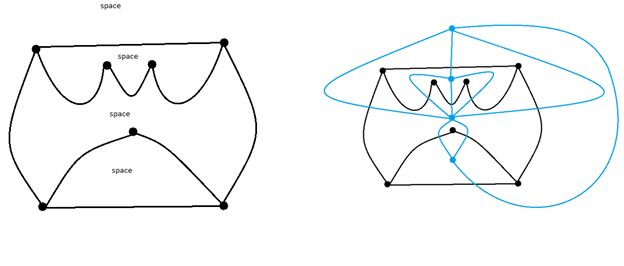
\includegraphics[scale=.7]{assets/josh/ghostplans}
\end{figure}

If Transylvania Plan D has 33 roads what is the cost of constructing the ghost city?

If the length of a space is the number of roads the space touches what is the sum of lengths of spaces in Plan D?
